\documentclass{standalone}
\usepackage{tikz}
\usepackage{ctex,siunitx,ninecolors}
\usepackage{tkz-euclide}
\usepackage{amsmath}
\usetikzlibrary{patterns, calc}
\usetikzlibrary {decorations.pathmorphing, decorations.pathreplacing, decorations.shapes,decorations.markings}
\begin{document}
\small
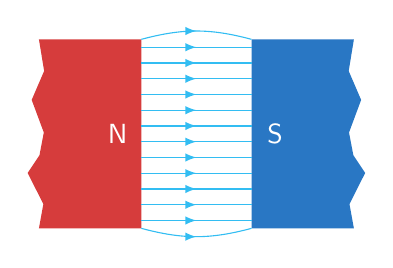
\begin{tikzpicture}[>=latex,scale=1.0]
  % \useasboundingbox(-1,-2)rectangle(8,6);
  \fill[red5](-2.0,1.2)--(-0.7,1.2)--(-0.7,-1.2)--(-2.0,-1.2)--(-1.944,-0.892)--(-2.143,-0.497)--(-1.993,-0.271)--(-1.938, 0.017)--(-2.092, 0.431)--(-1.934, 0.798)--cycle;
  \fill[azure5](2.0,1.2)--(0.7,1.2)--(0.7,-1.2)--(2.0,-1.2)--(1.944,-0.892)--(2.143,-0.497)--(1.993,-0.271)--(1.938, 0.017)--(2.092, 0.431)--(1.934, 0.798)--cycle;
  \node at (-1,0)[text=white]{\sffamily N};
  \node at (1,0)[text=white]{\sffamily S};
  \foreach \x in {-1.1,-0.9,...,1.2}
    {
      \draw[cyan!80!white,postaction={decorate},decoration={markings,mark={at position 0.5 with {\arrow{>}} }}](-0.7,\x)--(0.7,\x);
    }
  \draw[cyan!80!white,postaction={decorate},decoration={markings,mark={at position 0.5 with {\arrow{>}} }}](-0.7,1.2)to[bend left=15](0.7,1.2);
  \draw[cyan!80!white,postaction={decorate},decoration={markings,mark={at position 0.5 with {\arrow{>}} }}](-0.7,-1.2)to[bend right=15](0.7,-1.2);
\end{tikzpicture}
\end{document}